\section{Results
\label{sec:results}}

The results of these searches are published in Ref. \cite{CMS-EXO-12-032-PLB}. The numbers of observed events and expected signal and background events after the final selections for the leptoquark and top squark searches are listed in Tables \ref{Res:tab:STyieldLQ} and \ref{Res:tab:STyieldLQD321}, respectively, and the selection efficiencies for the two signals are listed in Tables~\ref{Res:tab:effLQ} and \ref{Res:tab:effLQD321}. The \ST distributions of the selected events from the observed data and from the background predictions, combining the \etau and \mutau channels, are shown in Fig. \ref{Res:fig:STfinalLQ} for the leptoquark search and Fig. \ref{Res:fig:STfinalLQD321} for the top squark search. The distribution from the 500\GeV (300\GeV) signal hypothesis is added to the background in Fig. \ref{Res:fig:STfinalLQ} (Fig. \ref{Res:fig:STfinalLQD321}) to illustrate how a hypothetical signal would appear above the background prediction. There is good agreement between the observed data and the SM background prediction.

An upper bound at the 95\% confidence level (CL) is set on $\sigma \mathcal{B}^2$. In the leptoquark search, $\sigma$ is the cross section for pair production of third-generation LQs and $\mathcal{B}$ is the branching fraction for the decay $\text{LQ} \rightarrow \tau \cPqb$. In the top squark search, $\sigma$ is the cross section for pair production of top squarks and $\mathcal{B}$ is the branching fraction for the decay $\sTop \rightarrow \chipm\cPqb, \chipm \rightarrow \sNu\tau^{\pm} \rightarrow \cPq\cPq\tau^{\pm}$. The modified-frequentist construction CL$_\mathrm{s}$ \cite{Read:presentation,Junk,LHC-HCG} is used for the limit calculation. A maximum likelihood fit is performed to the \ST distribution simultaneously for the \etau and \mutau channels, taking into account correlations between the systematic uncertainties. Appendix \ref{ch:limits} contains more details on the computation of CL$_\mathrm{s}$ limits using a distribution. The expected and observed upper limits on $\sigma \mathcal{B}^2$ as a function of the signal mass are shown in Fig.~\ref{Res:fig:asymptoticCombLQ} for the leptoquark search and Fig.~\ref{Res:fig:asymptoticCombLQD} for the top squark search.

We extend the current limits and exclude scalar leptoquarks and top squarks decaying through the coupling $\lambda^{\prime}_{333}$ with masses below 740\GeV, in agreement with the expected limit of 750\GeV. We exclude top squarks undergoing a chargino-mediated decay involving the coupling $\lambda^{\prime}_{3jk}$ with masses in the range 200--580\GeV, in agreement with the expected limit in the range 200--590\GeV. These upper limits assume $\mathcal{B}=100\%$. Similar results are obtained when calculating upper bounds using a
Bayesian method with a uniform positive prior for the cross section.

The upper bounds for the leptoquark search as a function of the leptoquark branching fraction and mass are shown in Fig.~\ref{Res:fig:2DCombLQ}. Small $\mathcal{B}$ values are not constrained by this search. Results from the CMS experiment on a search for top squarks decaying to a top quark and a neutralino \cite{SUS-13-011} are used to improve the constraints on $\mathcal{B}$. If the neutralino is massless, the final state kinematic distributions for such a signal are the same as those for the pair production of leptoquarks decaying to a tau neutrino and a top quark. Limits can therefore be placed on this signal, which must have a branching fraction of $1-\mathcal{B}$ if the leptoquark only decays to third-generation fermions. This reinterpretation is included in Fig.~\ref{Res:fig:2DCombLQ}. The unexcluded region at $\MLQ=200$--230\GeV corresponds to a portion of phase space where it is topologically very difficult to distinguish between the top squark signal and the \ttbar process, due to small \met. A top squark excess in this region would imply an excess in the measured \ttbar cross section of ${\sim}10\%$.

\begin{table}[htbp]
  \centering
    \begin{tabular}{|l|r@{$\,\pm\,$}r@{$\,\pm\,$}r|r@{$\,\pm\,$}r@{$\,\pm\,$}r|}
      \cline{2-7}
      \multicolumn{1}{l|}{} & \multicolumn{3}{c|}{\etau} & \multicolumn{3}{c|}{\mutau} \\
      \hline
      \ttbar irreducible              &  \multicolumn{1}{r@{\hphantom{$\,\pm\,$}}}{105.6} & & 18.1 &  \multicolumn{1}{r@{\hphantom{$\,\pm\,$}}}{ 66.7} & & 12.6  	    \\
      Major reducible                 &  \multicolumn{1}{r@{\hphantom{$\,\pm\,$}}}{147.8} & & 33.0 &  \multicolumn{1}{r@{\hphantom{$\,\pm\,$}}}{117.3} & & 18.9  	    \\
      Z($\ell\ell$/$\tau\tau$) + jets &    21.4 & 7.4 & 4.9   &    7.5 & 4.6 & 0.2  \\
      Single t                        &   16.0 & 2.8 & 4.4    &   17.3 & 2.8 & 4.7  \\
      VV                              &   4.1 & 0.6 & 1.3     &    2.6 & 0.5 & 0.8  \\
      \hline
      Total exp. bkg.                 & 294.9 & 7.9 & 39.1    & 211.4 & 5.4 & 23.4   \\
      \hline
      Observed                        & \multicolumn{1}{r@{\hphantom{$\,\pm\,$}}}{289\hphantom{.1}} & \multicolumn{1}{r}{} & \multicolumn{1}{r|}{} & \multicolumn{1}{r@{\hphantom{$\,\pm\,$}}}{216\hphantom{.1}} & \multicolumn{1}{r}{} & \multicolumn{1}{r|}{} \\
      \hline
     $\MLQ=500\GeV$                   & 57.7 & 1.4 & 5.9      & 51.6 & 1.3 & 5.3    \\
     $\MLQ=600\GeV$                   & 20.1 & 0.5 & 1.9      & 17.7 & 0.4 & 1.6    \\
     $\MLQ=700\GeV$                   & 7.1 & 0.2 & 6.3       & 6.2 & 0.1 & 5.5    \\
     $\MLQ=800\GeV$                   & 2.7 & 0.1 & 0.2       & 2.3 & 0.1 & 0.2    \\
      \hline
    \end{tabular}
    \caption{The estimated backgrounds, observed event yields, and expected number of signal events for the leptoquark search. For the simulation-based entries, the statistical and systematic uncertainties are shown separately, in that order. Only the systematic uncertainties are shown for the data-driven background entries.}    
    \label{Res:tab:STyieldLQ}
\end{table}

\begin{table}[htbp]
  \centering
    \begin{tabular}{|l|r@{$\,\pm\,$}r@{$\,\pm\,$}r|r@{$\,\pm\,$}r@{$\,\pm\,$}r|}
      \cline{2-7}
      \multicolumn{1}{l|}{} & \multicolumn{3}{c|}{\etau} & \multicolumn{3}{c|}{\mutau} \\
      \hline
      \ttbar irreducible              & \multicolumn{1}{r@{\hphantom{$\,\pm\,$}}}{88.3} & & 13.7 &  \multicolumn{1}{r@{\hphantom{$\,\pm\,$}}}{55.0} & & 9.5           \\
      Major reducible                 & \multicolumn{1}{r@{\hphantom{$\,\pm\,$}}}{65.7} & & 16.4 &  \multicolumn{1}{r@{\hphantom{$\,\pm\,$}}}{59.8} & & 13.8          \\
      Z($\ell\ell$/$\tau\tau$) + jets & 4.9 & 2.5 & 1.1      &  11.6 & 5.5 & 2.7   \\
      Single t                        & 3.9 & 1.5 & 1.1      &  3.5 & 1.3 & 0.9   \\
      VV                              & 0.6 & 0.2 & 0.2      &  0.4 & 0.2 & 0.1   \\
      \hline
      Total exp. bkg.                 & 163.4 & 2.9 & 21.5   & 130.3 & 5.6 & 17.1 \\
      \hline
      Observed                        & \multicolumn{1}{r@{\hphantom{$\,\pm\,$}}}{156\hphantom{.1}} & \multicolumn{1}{r}{} & \multicolumn{1}{r|}{} & \multicolumn{1}{r@{\hphantom{$\,\pm\,$}}}{123\hphantom{.1}} & \multicolumn{1}{r}{} & \multicolumn{1}{r|}{} \\
      \hline
      $\Mstop=300\GeV$                & 94.3 & 8.5 & 13.2    &  82.8 & 8.0 & 11.7  \\
      $\Mstop=400\GeV$                & 43.9 & 2.6 & 4.3     &  38.3 & 2.3 & 3.8   \\
      $\Mstop=500\GeV$                & 19.4 & 0.8 & 1.8     &  15.4 & 0.7 & 1.5   \\
      $\Mstop=600\GeV$                & 6.9 & 0.9 & 0.7      &   5.7 & 0.3 & 0.5   \\
      \hline
    \end{tabular}
    \caption{The estimated backgrounds, observed event yields, and expected number of signal events for the top squark search. For the simulation-based entries, the statistical and systematic uncertainties are shown separately, in that order. Only the systematic uncertainties are shown for the data-driven background entries.}
    \label{Res:tab:STyieldLQD321}
\end{table}

\begin{table}[htbp]
  \centering
    \begin{tabular}{|l|r|r|r|r|r|r|r|r|r|}
      \hline
      \MLQ (\GeVns) & 200 & 250 & 300 & 350 & 400 & 450 & 500 & 550 & 600  \\
      \hline
      \etau  & 0.1 & 0.3 & 1.0 & 1.9 & 2.4 & 3.0 & 3.6 & 4.0 & 4.4  \\
      \mutau & 0.1 & 0.2 & 0.8 & 1.5 & 2.3 & 2.9 & 3.2 & 3.3 & 3.8   \\
      \hline
      \noalign{\vskip 2pt} 
      \cline{1-9}
      \MLQ (\GeVns) & 650 & 700 & 750 & 800 & 850 & 900 & 950 & 1000 & \multicolumn{1}{r}{} \\
      \cline{1-9}
      \etau  & 4.5 & 4.7 & 4.9 & 5.1 & 5.4 & 5.1 & 5.4 & 5.5 & \multicolumn{1}{r}{} \\
      \mutau & 4.0 & 4.1 & 4.2 & 4.3 & 4.4 & 4.4 & 4.3 & 4.4 & \multicolumn{1}{r}{} \\
      \cline{1-9}
    \end{tabular}
    \caption{Selection efficiencies in \% for the signal in the leptoquark search, estimated from the simulation.}
    \label{Res:tab:effLQ}
\end{table}

\begin{table}[htbp]
  \centering
    \begin{tabular}{|l|r|r|r|r|r|r|r|r|}
      \hline
      \Mstop (\GeVns) & 200 & 300 & 400 & 500 & 600 & 700 & 800 & 900 \\
      \hline
      \etau  & 0.02 & 0.3 & 0.7 & 1.2 & 1.5 & 1.8 & 1.8 & 1.5 \\
      \mutau & 0.02 & 0.2 & 0.6 & 1.0 & 1.2 & 1.4 & 1.3 & 1.1 \\
      \hline
    \end{tabular}
    \caption{Selection efficiencies in \% for the signal in the top squark search, estimated from the simulation.}
    \label{Res:tab:effLQD321}
\end{table}

\begin{figure}[htbp]
  \centering
    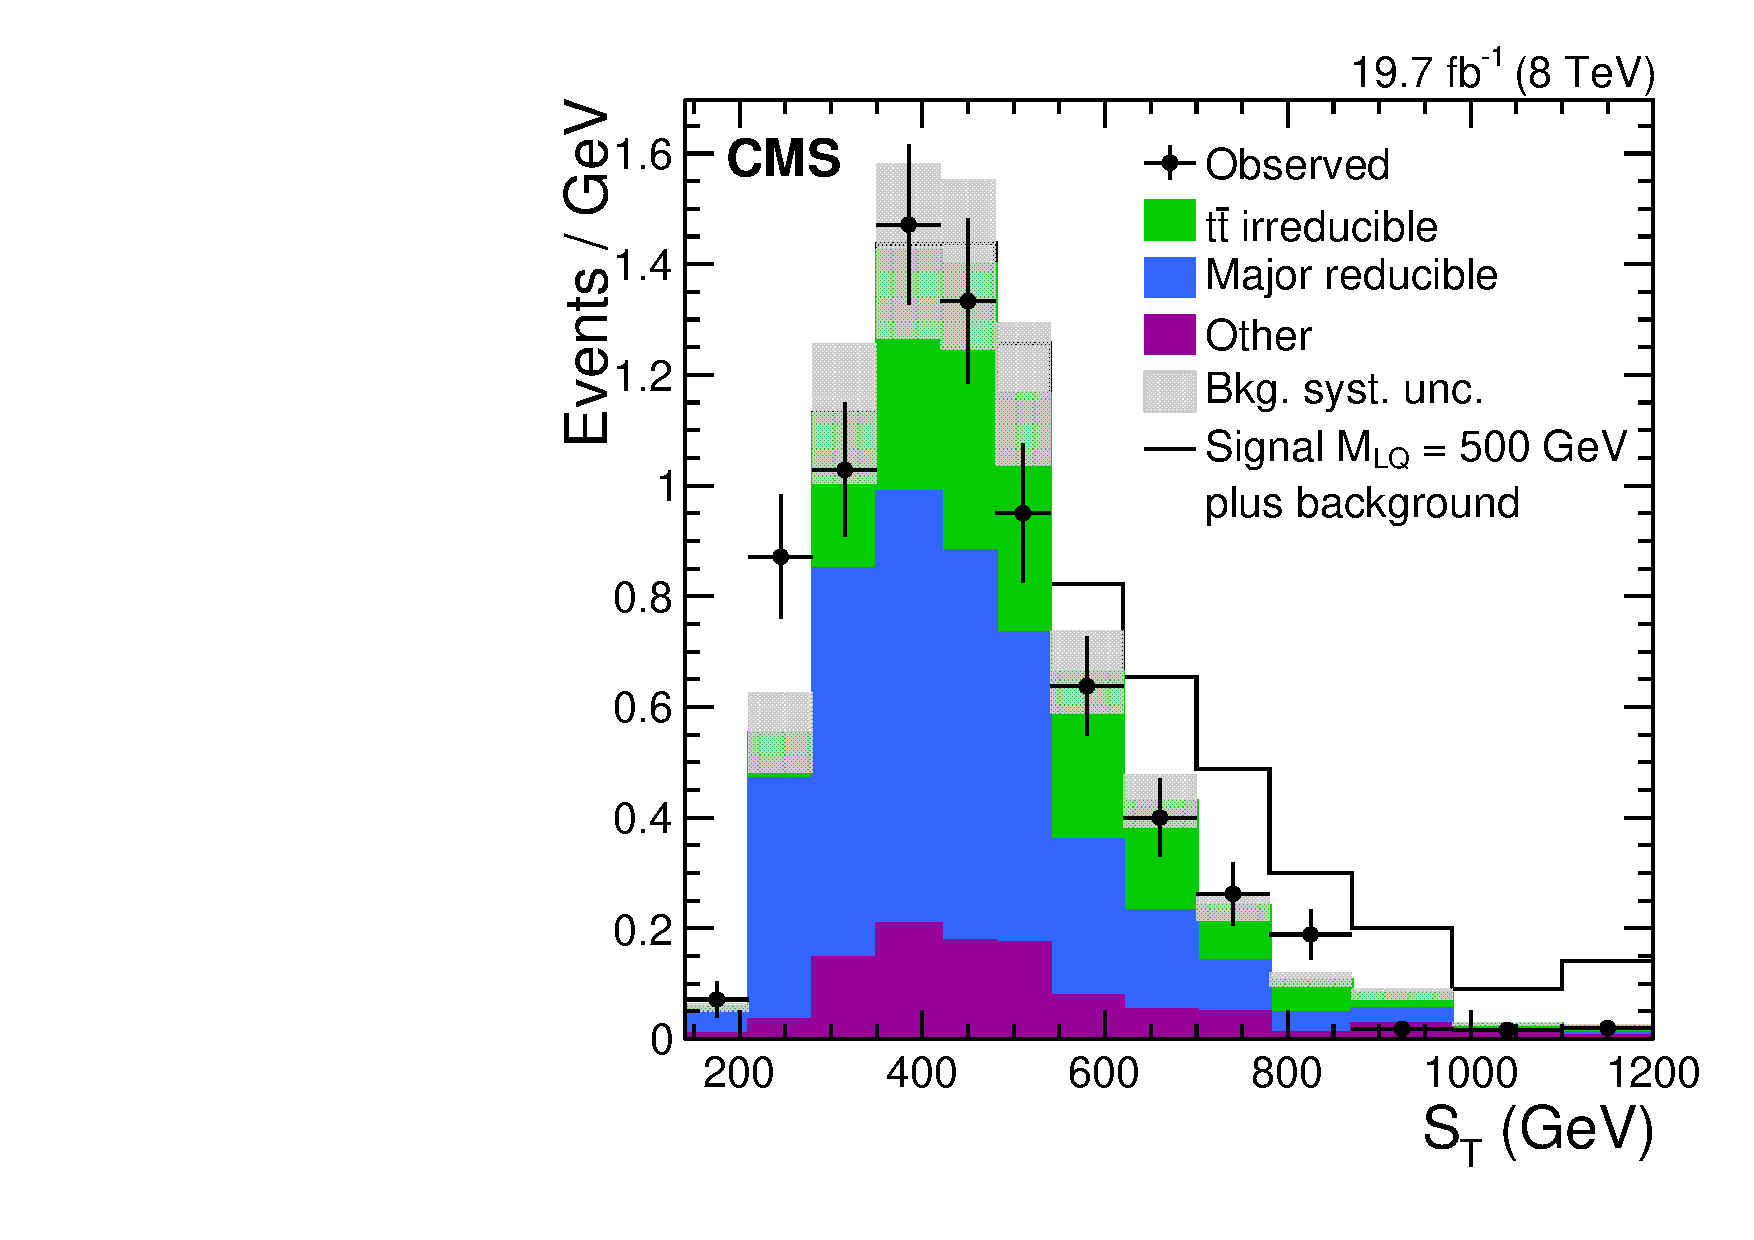
\includegraphics[width=0.7\textwidth]{figures/final/st_lq.pdf}
    \caption{The final \ST distribution for the leptoquark search with the \etau and \mutau channels combined.
             A signal sample for leptoquarks with $\MLQ=500\GeV$ is added on top of the background prediction.
             The last bin contains the overflow events. The horizontal bar on each observed data point indicates the width of the bin in \ST.
           }
    \label{Res:fig:STfinalLQ}
\end{figure}

\begin{figure}[htbp]
  \centering
    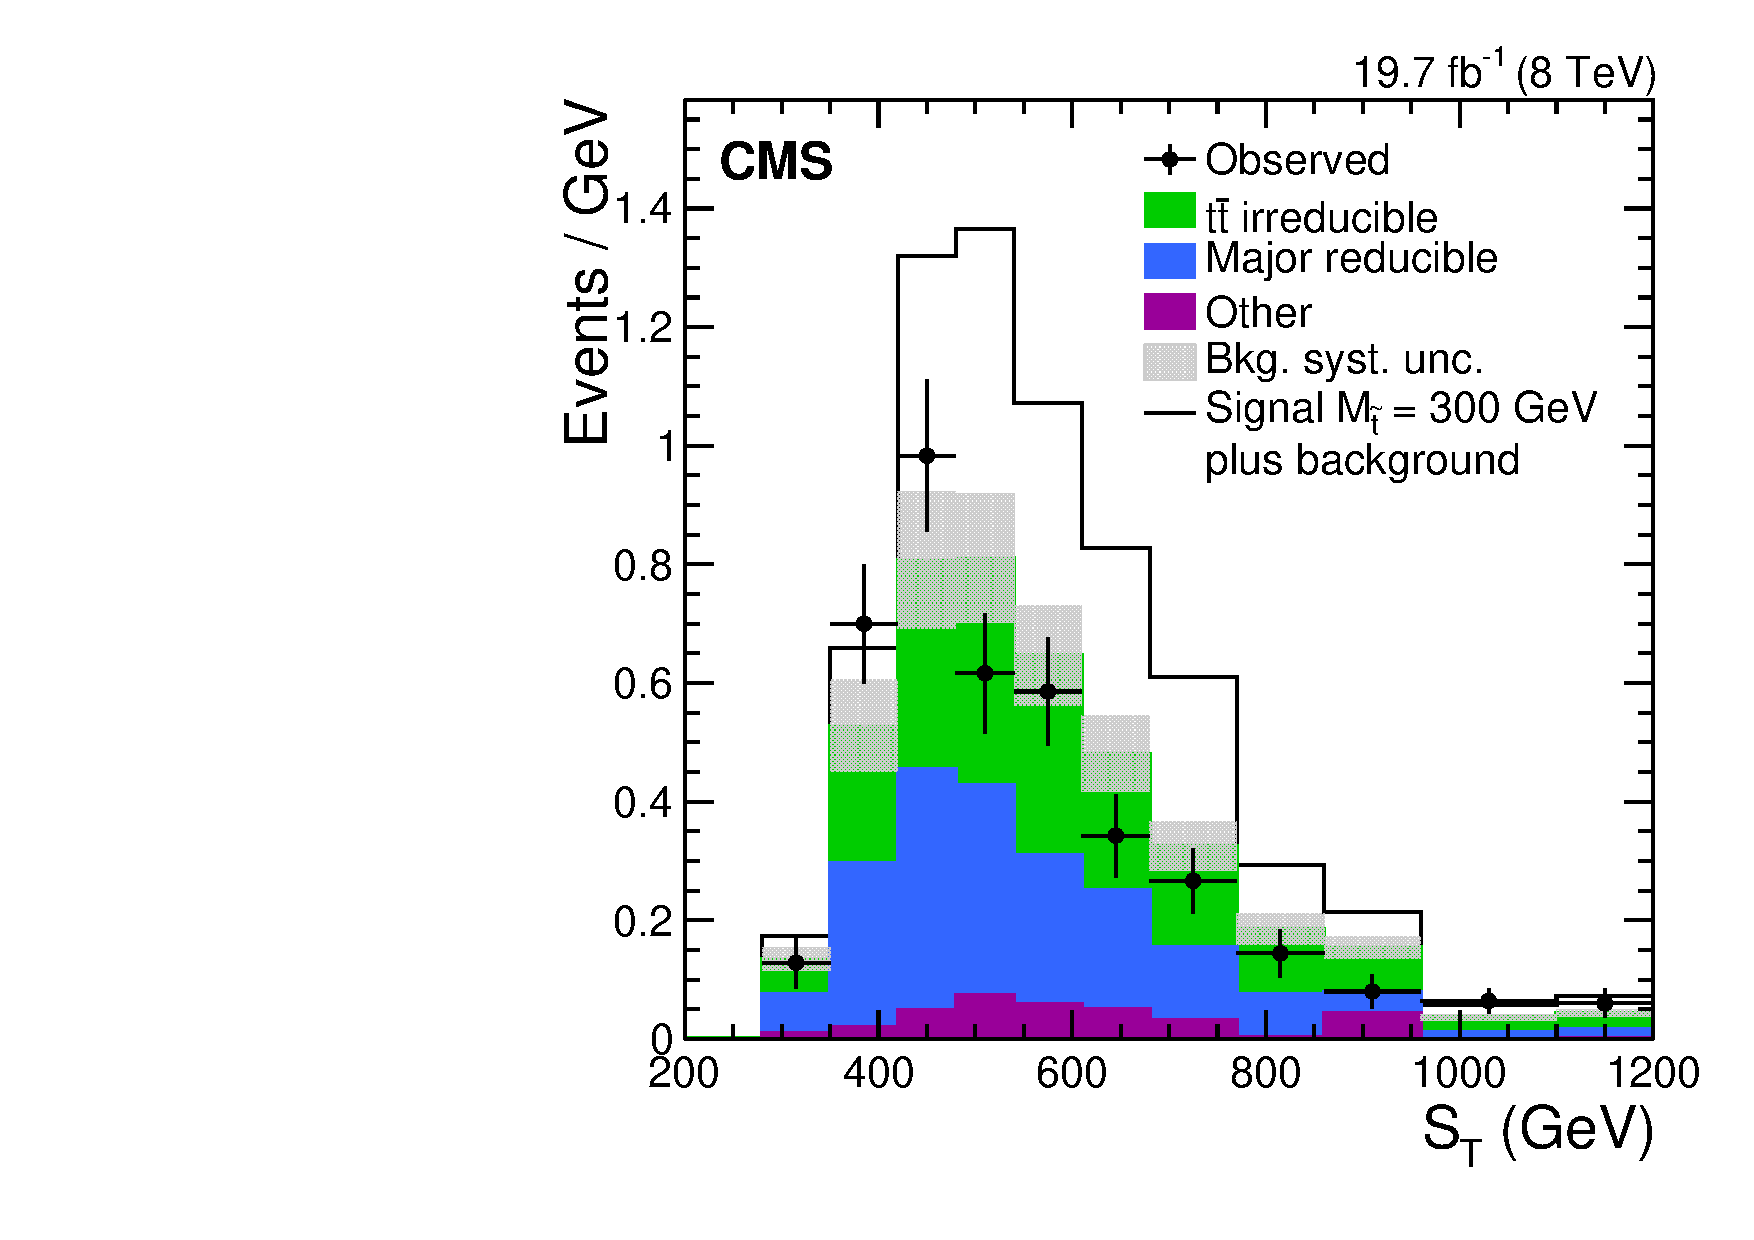
\includegraphics[width=0.7\textwidth]{figures/final/st_lqd321.pdf}
    \caption{The final \ST distribution for the top squark search with the \etau and \mutau channels combined.
             A signal sample for top squarks with $\Mstop=300\GeV$ is added on top of the background prediction.
             The last bin contains the overflow events. The horizontal bar on each observed data point indicates the width of the bin in \ST.
           }
    \label{Res:fig:STfinalLQD321}
\end{figure}

\begin{figure}[htbp]
  \centering
    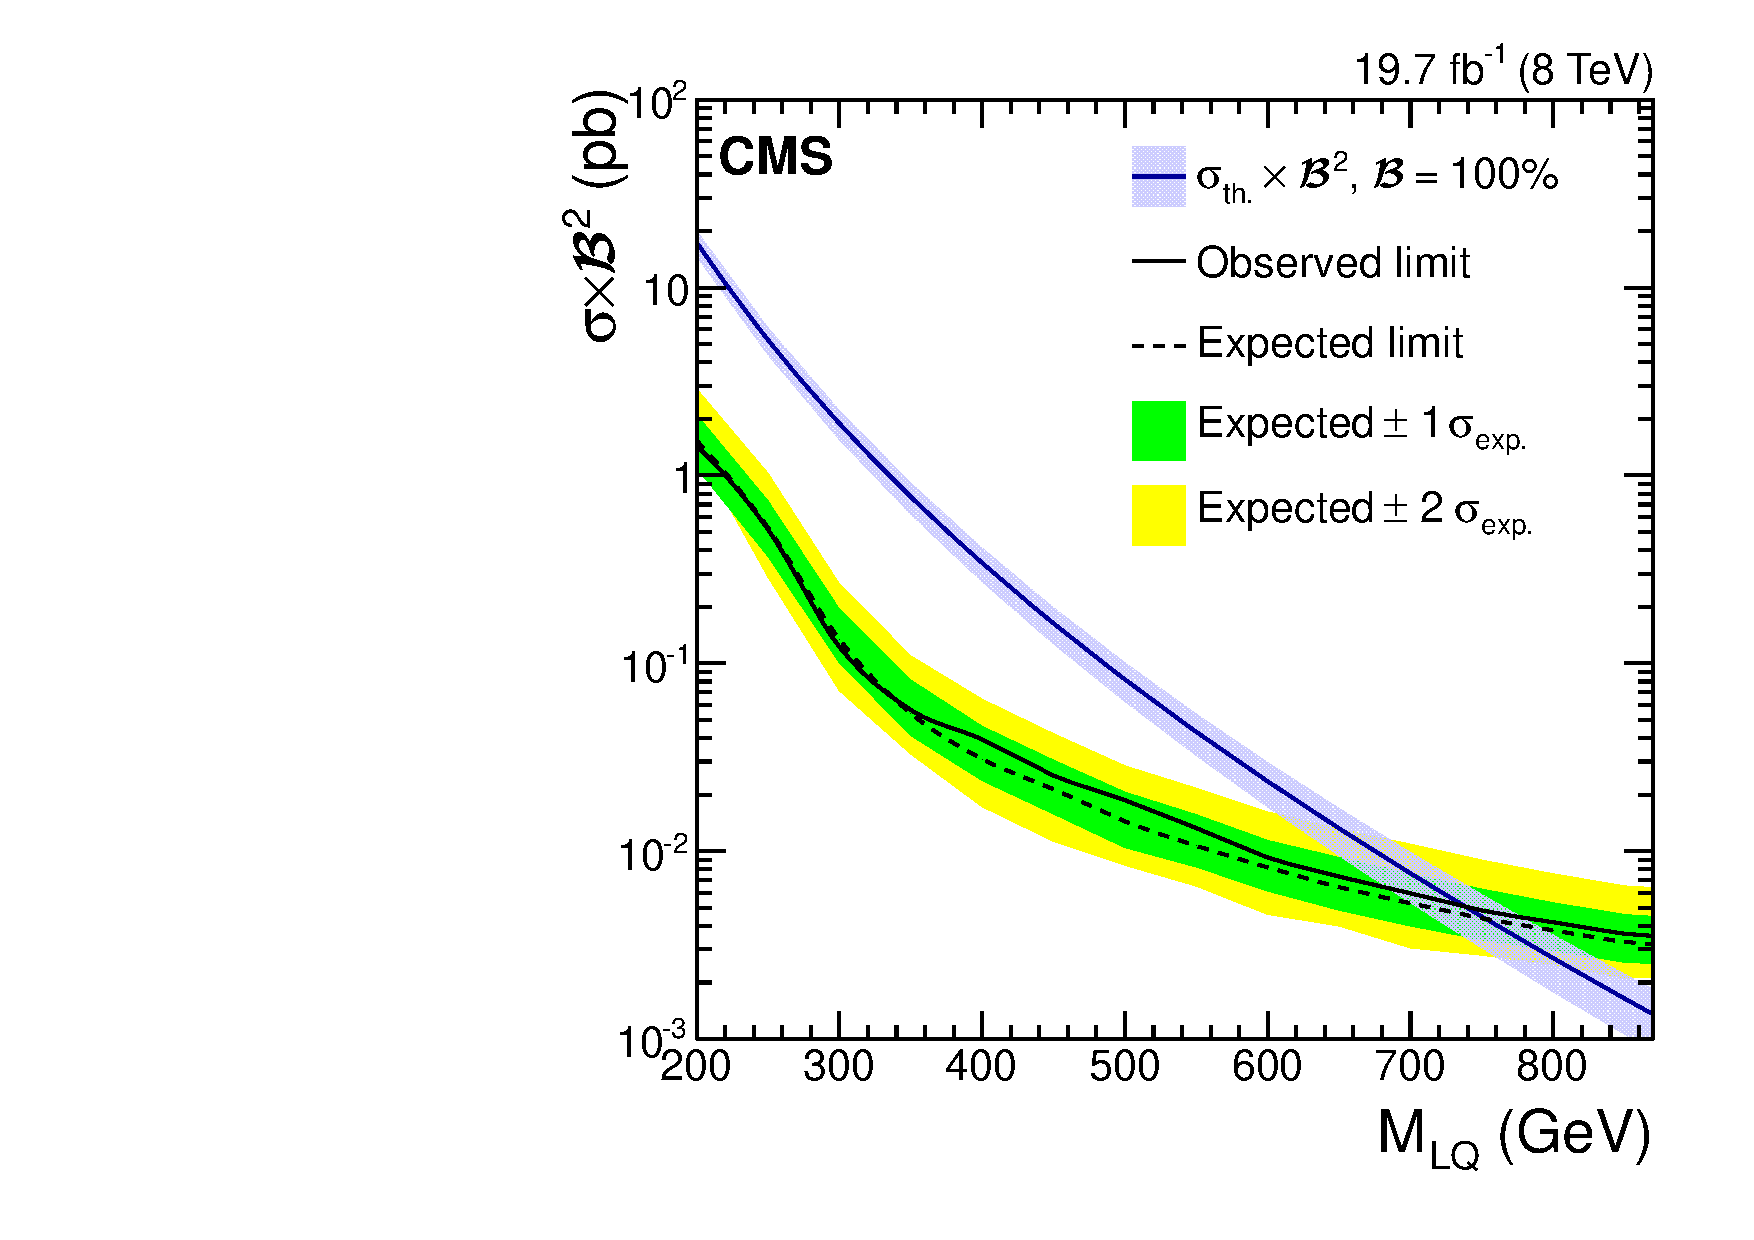
\includegraphics[width=0.7\textwidth]{figures/final/BR_Sigma_TauTau_LQ.pdf}
    \caption{The expected and observed combined upper limits on the third-gen\-er\-a\-tion LQ pair production cross section $\sigma$ times the square of the branching fraction, $\mathcal{B}^2$, at the 95\% CL, as a function of the LQ mass. These limits also apply to top squarks decaying directly via the coupling $\lambda^{\prime}_{333}$. The green (darker) and yellow (lighter) uncertainty bands represent the 68\% and 95\% CL intervals on the expected limit. The dark blue curve and the hatched light blue band represent the theoretical LQ pair production cross section, assuming $\mathcal{B}=100\%$, and the uncertainties due to the choice of PDF and renormalization/factorization scales.}
    \label{Res:fig:asymptoticCombLQ}
\end{figure}

\begin{figure}[htbp]
\centering
    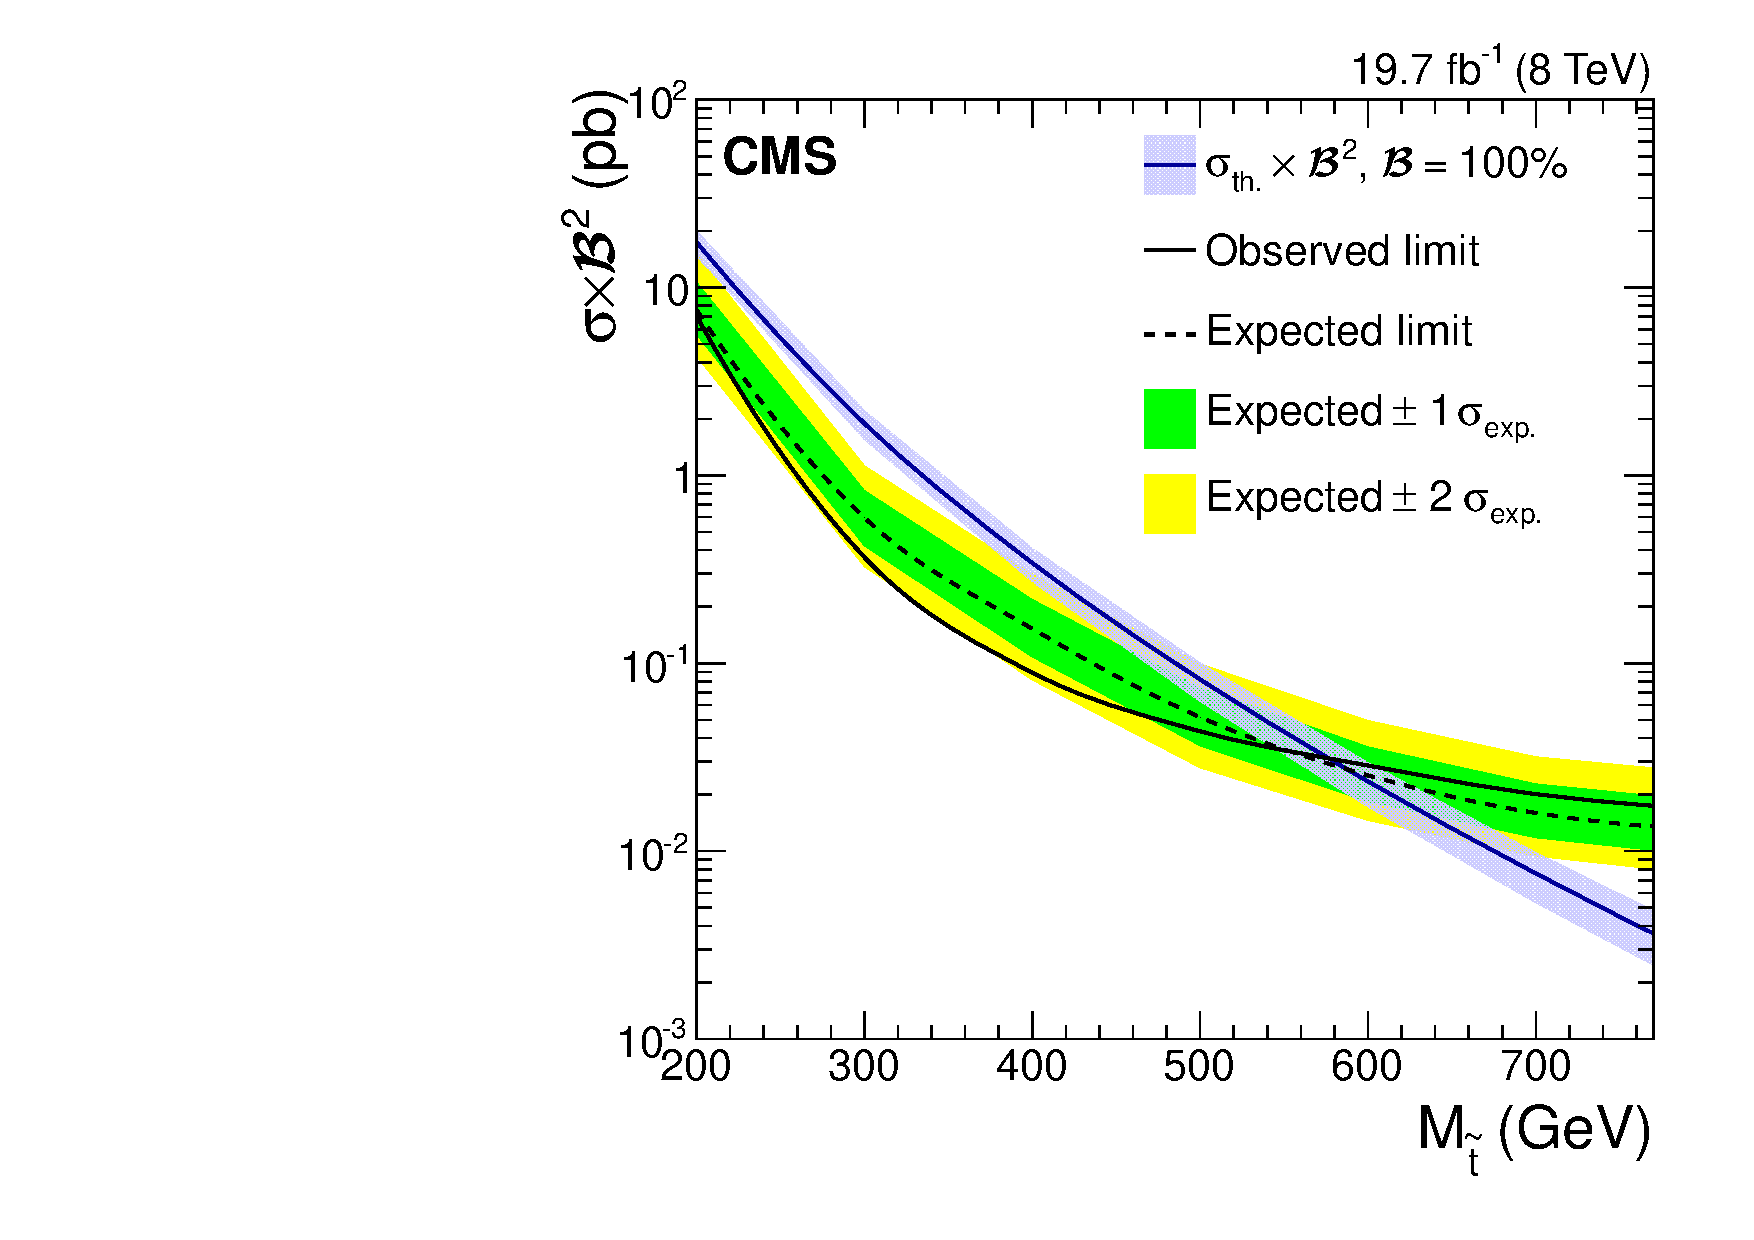
\includegraphics[width=0.7\textwidth]{figures/final/BR_Sigma_TauTau_LQD.pdf}
    \caption{The expected and observed combined upper limits on the top squark pair production cross section $\sigma$ times the square of the branching fraction, $\mathcal{B}^2$, at the 95\% CL, as a function of the top squark mass. These limits apply to top squarks with a chargino-mediated decay through the coupling $\lambda^{\prime}_{3kj}$. The green (darker) and yellow (lighter) uncertainty bands represent the 68\% and 95\% CL intervals on the expected limit. The dark blue curve and the hatched light blue band represent the theoretical top squark pair production cross section, assuming $\mathcal{B}=100\%$, and the uncertainties due to the choice of PDF and renormalization/factorization scales.}
    \label{Res:fig:asymptoticCombLQD}
\end{figure}

\begin{figure}[htbp]
\centering
    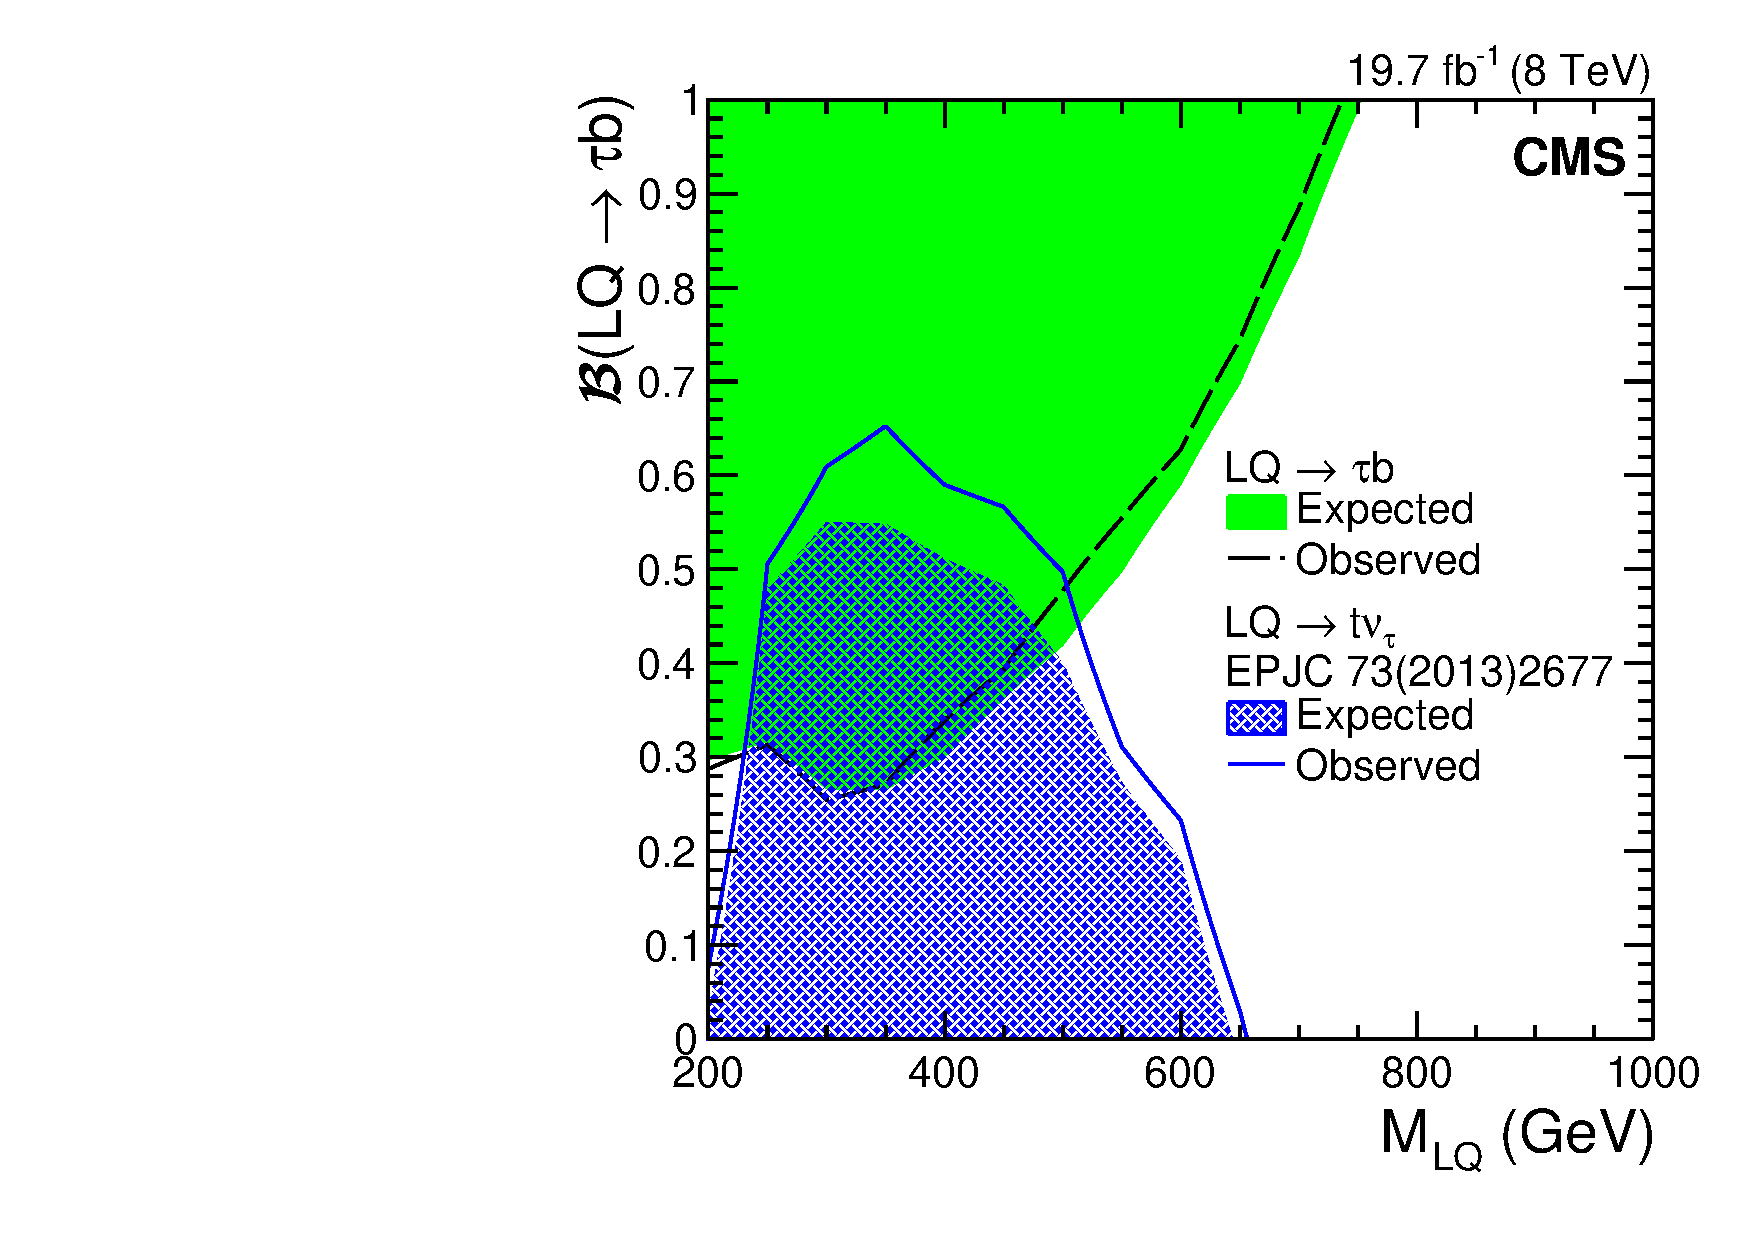
\includegraphics[width=0.7\textwidth]{figures/final/limit_beta_vs_mass_btau_topnu.pdf}
    \caption{The expected (dashed black) and observed (green solid) 95\% CL upper limits on the branching fraction for the leptoquark decay to a tau lepton and a bottom quark, as a function of the leptoquark mass. A search for top squark pair production \cite{SUS-13-011} has the same kinematic signature as the leptoquark decay to a tau neutrino and a top quark. This search is reinterpreted to provide the expected (blue hatched) and observed (blue open) 95\% CL upper limits for low values of $\mathcal{B}$, assuming the leptoquark only decays to third-generation fermions.}
    \label{Res:fig:2DCombLQ}
\end{figure}